\documentclass[openany, a4, 11pt]{book}

% Documentul va fi tradus in limba romana
\usepackage[romanian]{babel}

% Scriem cu diacritice... 
\usepackage[utf8x]{inputenc}

% Vom folosi si un appendix simplut
\usepackage[toc,page]{appendix}

% Se importa si pachetul pentru URL-uri (acestea vor fi colorate cu albastru)
\usepackage{hyperref}
\usepackage[pdftex]{graphicx}    
\usepackage{subfig}
\usepackage{multicol}
\usepackage{color}
\usepackage{indentfirst}
\usepackage{pifont}
\usepackage[margin=2.8cm, vmargin={1.4in, 1.4in}]{geometry}
% \usepackage[bindingoffset=0.2in, left=1.0in, right=1.0in]{geometry}

% Pachetele necesare pentru crearea si afisarea formulelor matematice
\usepackage{mathtools}

% Folosim un pachet pentru antet si subsol
\usepackage{fancyhdr}
\pagestyle{fancy}

% Pachetele necesare pentru listarea de cod sursa
\usepackage{caption}
\usepackage{listings}
\usepackage{xcolor}

% Pachetele necesare pentru crearea unor casute cu diverse mesaje
\usepackage{styles/boxes}

\usepackage{array}
\usepackage{booktabs}
\usepackage{multirow}

% Pachete necesare pentru desenarea unor figuri pe ecranul utilizatorului
\usepackage{wrapfig}
\usepackage{graphicx}
\usepackage{subfig}

% Importam si pachetul necesar pentru QR code
\usepackage[]{qrcode}

\definecolor{gray}{RGB}{235,235,235}
\definecolor{codegreen}{rgb}{0,0.6,0}
\definecolor{codegray}{rgb}{0.5,0.5,0.5}
\definecolor{codepurple}{rgb}{0.58,0,0.82}
\definecolor{backcolour}{rgb}{0.95,0.95,0.92}

\renewcommand*\lstlistingname{Cod sursă}

% Numele paginii de Aneze din cuprins este redenumit
\renewcommand{\appendixtocname}{Anexă}

% Legaturile web vor fi colorate cu albastru
\newcommand{\myhref}[3][blue]{\href{#2}{\color{#1}{#3}}}%

% Alte modificari de configurare
\renewcommand{\headrulewidth}{1pt}
\renewcommand{\footrulewidth}{1pt}
\setlength{\headheight}{12pt}
\setcounter{secnumdepth}{6}
% Adancimea cuprinsului...
\setcounter{tocdepth}{3}
% Seteaza identarea unui paragraf
\setlength{\parindent}{1cm}

% Pentru cuprins se scoate culoarea si bordarea legaturilor
\hypersetup{urlbordercolor={1 1 1}, linkbordercolor={1 1 1}, citebordercolor={1 1 1}}

% De aici incepe documentul nostru!
\begin{document}

\newgeometry{margin=3cm}
\begin{titlepage}

% Titlul va aparea centrat
\begin{center}
 
\begin{figure}[htb]
\center{

\includegraphics[width=0.4 \textwidth]{images/freescale_logo.png}
}
\end{figure}
\noindent{\rule{8cm}{0.4pt}}\\[0.3cm]
\textsc{\Large STEM Innovation Champ}\\[5.0cm]

{\Huge DOCUMENTAȚIE}\\[0.4cm]
\textsc{\Large Utilă pentru realizarea unui robot de tip\\ LINE FOLLOWER}\\[5.0cm]

% Informatii despre autor si despre indrumator
\begin{minipage}{0.5\textwidth}
\begin{flushleft}
\large{\textbf{Ediție concurs}}\\
\large{a 2-a (martie 2015)}
\end{flushleft}
\end{minipage}
~
\begin{minipage}{0.4\textwidth}
\begin{flushright}
\large{\textbf{Revizie document}} \\
1.0\\
\end{flushright}
\end{minipage}\\[3.0cm]

% Alte informatii aditionale?
\noindent{\rule{8cm}{0.4pt}}\\[0.3cm] 
{\large martie 2015}\\[1cm] 

\end{center}

% Trecem la urmatoarea pagina...
\end{titlepage}
\restoregeometry

% Cine a contribuit la acest proiect?
%\newgeometry{margin=5cm}
%\thispagestyle{empty}
%\section*{\centering{Listă de schimbări}}
%\restoregeometry

% Setarile necesare pentru a include cod sursa in cadrul acestei documentatii
\lstdefinestyle{customc}{
    backgroundcolor=\color{backcolour},   
    commentstyle=\color{codegray},
    keywordstyle=\color{green!40!black},
    stringstyle=\color{codepurple},
    basicstyle=\footnotesize,
    numberstyle=\tiny\color{codegray},
    identifierstyle=\color{blue},
    belowcaptionskip=1\baselineskip,
    breaklines=true,
    language=C,
    showstringspaces=false,
    captionpos=b,                    
    keepspaces=true,                 
    numbers=left,                    
    numbersep=5pt,                  
    showspaces=false,                
    showstringspaces=false,
    showtabs=false,                  
    tabsize=2
}

% Sectiunea "Abstract"
\newgeometry{margin=5cm}
\thispagestyle{empty}
\begin{multicols}{2}
[
\section*{Cuvânt înainte,}
]
\footnotesize {
Documentul de față își propune să vă ajute pe parcursul desfășurării proiectului \textit{"Line Follower"} organizat de \textit{Freescale România} în parteneriat cu \textit{Junior Achievement România}.

Dorim să vă informăm, de la bun început, de faptul că limbajul sau anumiți termeni ce apar în cadrul acestui document s-ar putea să nu vă fie familiari. Chiar dacă acest lucru se întâmplă, nu trebuie să vă panicați pentru că multe din aceste informații vă vor fi prezentate la sedințele tehnice pe care le veți avea cu mentorii. De fapt, prima ședință chiar asta îți propune: să aducă întreagă echipa la același nivel de cunoștințe și să aibă un vocabular adecvat. În celelalte trei ședințe ne vom ocupa de scris cod și optimizat soluția, dar începutul e cel mai important.

Vă recomandăm să citiți acest document înainte de a avea loc discuțiile cu mentorii. În acest fel, veți putea să vă faceți o idee despre ceea ce vom realiza, iar dacă ceva nu vă este clar, vă invităm să pregătiți o listă de întrebări pentru mentorii voștri.

Ce vei găsi în materialul de față? În primul rând, se vor regăsi explicații teoretice / fizice prin care se demonstrează modul de funcționare a unor module hardware și cum acestea pot fi programate folosind o unealtă ajutătoare. În al doilea rând, vei fi introdus în lumea sistemelor embedded, vei învăța cum poți controla un dispozitiv prin intermediul unui algoritm transpus într-un limbaj de programare, precum C.

}
\end{multicols}
\begin{flushright}\textit{Mult succes,\\Mentorii Freescale}\end{flushright}
\restoregeometry

% Se afiseaza si un cuprins avansat
\tableofcontents

% Pagina cu lista de figuri
\renewcommand\listfigurename{Listă de figuri}
\listoffigures

% Sectiunea de introducere
\chapter{Sisteme încorporate}

Termenul de \textit{sistem încorporat} reprezintă traducerea în limba română a \textit{embedded system} și semnifică un calculator de mici dimensiuni bazat pe un microprocesor, util în vederea îndeplinirii unei sarcini anume (foarte rar avem de-a face cu mai multe sarcini). În plus, se pune accentul pe posibilitatea procesării datelor și luarea unor decizii în timp real. Dacă la un calculatator personal este acceptabilă o întârziere de 2-3 secunde atunci când are loc încărcarea unei aplicații, în lumea embedded un lag de acest gen, poate conduce la pierderea ireversibilă a stării curente.

Un astfel de sistem poate acoperi o gamă largă de aplicații, fiind constituit din mai multe componente mecanice și electronice ce sunt interconectate și administrate de un modul cheie - un microcontroller. Acesta din urmă nu este altceva decât creierul, elementul prin care este insuflată inteligență dispozitivului pe care îl creăm. Ca și definiție, microcontroller-ul este un chip (circuit integrat) ce încorporează o unitate centrală (CPU) și o memorie împreună cu resurse care-i permit interacțiunea cu mediul exterior (interacțiunea cu mediul exterior se va realiza prin intermediul unor senzori).

Microcontrollerele sunt utilizate în foarte multe domenii, dintre care am enumera: industria de automobile (controlul aprinderii motorului, climatizare, diagnoză, sisteme de alarmă, computer de bord), în așa zisa electronică de consum (sisteme audio, televizoare, camere video și videocasetofoane, telefonie mobilă, GPS-uri, jocuri electronice), în aparatura electrocasnică (mașini de spălat, frigidere, cuptoare cu microunde, aspiratoare), în controlul mediului și climatizare (sere, locuințe, hale industriale), în industria aerospațială, în mijloacele moderne de măsurare - instrumentație (aparate de măsură, senzori și traductoare inteligente) cât și în medicină. Ca un exemplu din industria de automobile, numai la nivelul anului 1999, un BMW seria 7 utiliza 65 de microcontrolere, iar un Mercedes din clasa S utiliza 63 de microcontrolere. Practic, deși am prezentat ca exemple concrete numai sisteme robotice și mecatronice, este foarte greu de găsit un domeniu de aplicații în care să nu se utilizeze microcontrolerele.

% Dezvoltarea unei aplicatii in CodeWarrior for MCU
\chapter{CodeWarrior for MCU}

Prin intermediul utilitarului \textit{CodeWarrior} se pune la dispoziție un mediu complet de dezvoltare software pentru sistemele embedded. Cu ajutorul acestei suite puse la dispoziție de Freescale, se oferă un suport consistent în ceea ce privește dezvoltarea aplicației (inclusiv partea de depanare a ei) reducându-se timpul și efortul necesar programării unui dispozitiv embedded. CodeWarrior se bazează pe Eclipse și conține mai multe componente. În primul rând are inclus un sistem de build, un compiler și un debugger engine. Pentru utilizarea lui este necesară o licență. În cazul ședințelor tehnice ce vor avea loc, pe parcursul acestui concurs, veți beneficia de toate condițiile necesare utilizării cu succes al acestui utilitar.

De aproximativ un an de zile, Freescale a introdus și un tool similar pentru familia \textit{Kinetis} și anume \textit{Kinetis Design Studio} ce înglobează o serie de module open-source. Este soluția perfectă cu care puteți să continuați să dezvoltați propriile aplicații embedded după terminarea acestui concurs. În continuare, vom prezenta \textit{CodeWarrior} ca și tool pe care îl vom folosi, dar să știți că o dată ce v-ați familarizat cu acesta din urmă, o să fie la îndemână și experimentarea pe alte soluții - gen \textit{Kinetis Design Studio}.

Pentru programarea unui microcontroller se pot folosi diverse metode, dintre care programarea bazată pe interfaţa serială, folosirea unui programator ISP (\textit{In-System Programming}) ce foloseşte interfaţa serială SPI sau folosirea unui \textit{bootloader}. În cadrul acestui concurs vom folosi ultima variantă, un bootloader fiind un program încărcat la sfârşitul memoriei program a microcontroller-ului (de exemplu programat folosind un programator ISP). Execuţia codului încărcat astfel va începe din zona de boot.

\section{Programarea microcontroller-ului folosind OpenSDA}

OpenSDA este un firmware ce rulează pe un core independent, și anume un K20DX (produs tot de Freescale) și care pune la dispoziție bootloader-ul de care avem nevoie pentru a putea programa microcontroller-ul. Acest firmware se poate descărca de la adresa\footnote{\myhref{http://www.pemicro.com/opensda/}{http://www.pemicro.com/opensda/}}, el necesitând și programarea sa pe placă. Bineînțeles, în cazul plăcilor de dezvoltare pe care vi le punem la dispoziție, vom realiza noi această parte, plăcile având deja ultima versiune a firmware OpenSDA. Totuși dorim să vă prezentăm în continuare și cum puteți face această lucru voi înșiși acasă. Pașii pe care trebuie să îi urmați ar fi următorii:

\begin{wrapfigure}{r}{0.4\textwidth}
    \vspace{-25pt}
    \center{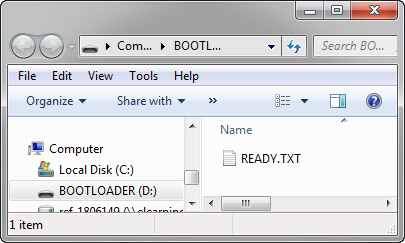
\includegraphics[width=0.4 \textwidth]{images/OSDevice.png}}
    \vspace{-20pt}
    \caption{\label{fig:CodeWarrior-OSDevice} Accesarea modului Bootloader}
    \vspace{-25pt}
\end{wrapfigure}

\begin{enumerate}
    \item Primul pas constă în intrarea în modulul \textit{Bootloader}, prin apăsarea butonului de \textit{Reset} în timp ce placa este alimentată de la sursă de tensiune. Mare atenție, pentru că alimentarea plăcii trebuie să se facă în timp ce acest buton este ținut apăsat.
    \item Confirmarea hardware pentru faptul că totul este bine și sunteți în acest mod, este oferită de un leg verde ce se află lângă modulul OpenSDA de pe Freedom board.
    \item În acest moment, dacă vă conectați calculatorul personal cu un cablu USB la Freedom board, sistemul de operare ar trebui să vă recunoască un nou device în sistem, așa cum este ilustrat în figura \ref{fig:CodeWarrior-OSDevice}.
    \item Folosind o simplă operație de tip drag \& drop se pot copia fișierele cu extensia SDA (ce au fost descărcate anterior) în cadrul device-ul ce se află în modul Bootloader. Procesul este asemănător cu cel al copierii unui fișier de pe o partiție pe alta.
    \item Un alt reset al plăcii (prin deconectarea și reconectarea la o sursă de alimentare) va produce începerea rulării fișierelor SDA încărcate la pasul anterior.
\end{enumerate}

După ce ați urmat toți pașii de mai sus, veți putea utiliza CodeWarrior fără probleme în programarea și depanarea programelor voastre. Aveți totuși grijă să creați un proiect având stabilită ca și conexiunea OpenSDA (și nu Segger spre exenmplu) pentru a-i putea specifica tool-ului modul de programare. Altfel, riscați să nu puteți programa placa!

Ajunți în acest punct, putem să începem să ne familarizăm cu mediul de dezvoltare și mai ales interfața pe care o oferă. Ați mai utilizat un IDE (\textit{Integrated Development Environment}) până acum?

\section{Vedere de ansamblu asupra utilitarului}

Figura \ref{fig:CodeWarrior-VedereDeAnsamblu} (de pe pagina următoare) ilustrează cele mai importante ferestre din mediul de dezvoltare \textit{CodeWarrior for MCU}. În partea de sus avem meniuri și butoane pentru acces rapid la anumite funcționalități, în stânga avem detalii legate de proiectele create și fișierele asociate lor, în centru ecranului apare un editor prin care se poate modifica conținutul fișierelor unui proiect, iar în partea de jos se poate observa dacă proiectul nostru conține erori. Acestea ar fi în mare câteva din elementele pe care le vom folosi, utilitarul punând la dispoziție o multitudine de feature-uri.

În cele ce urmează vor fi prezentate succint câteva dintre acțiunile cele mai des întâlnite pe care le veți realiza pe parcursul dezvoltării programului vostru.

\begin{figure}[h!]
    \vspace{-15pt}
    \center{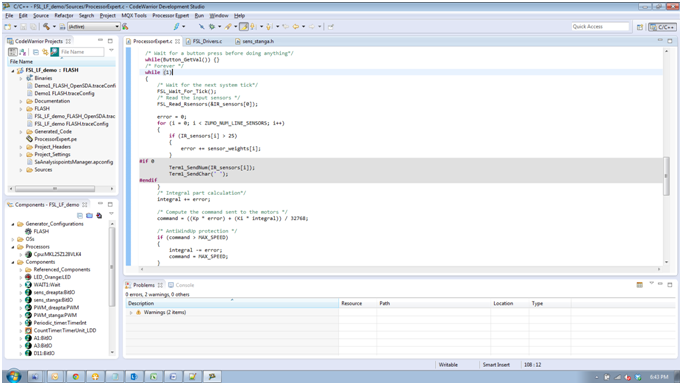
\includegraphics[width=1.0 \textwidth]{images/CodeWarriorMCU.png}}
    \vspace{-20pt}
    \caption{\label{fig:CodeWarrior-VedereDeAnsamblu} CodeWarrior for MCU - Vedere de ansamblu}
    \vspace{-10pt}
\end{figure}

\section{Compilarea proiectului}

\begin{wrapfigure}{r}{0.5\textwidth}
    \vspace{-50pt}
    \center{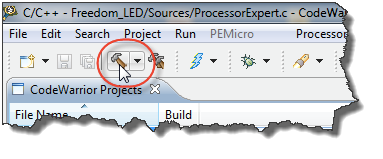
\includegraphics[width=0.5 \textwidth]{images/BuildProject.png}}
    \vspace{-30pt}
    \caption{\label{fig:CodeWarrior-CompilareProiect} Cum se poate compila proiectul}
    \vspace{-10pt}
\end{wrapfigure}

Pentru a compila proiectul, după ce în prealabil s-a generat codul folosind ProcessorExpert și voi v-ați scris codul vostru sursă, puteti folosi butonul din figura \ref{fig:CodeWarrior-CompilareProiect} sau de ce nu puteți folosi meniul principal și anume opțiunea \textit{Project $\rightarrow$ Build Project}. Indiferent de varianta aleasă rezultatul va fi același.

\begin{wrapfigure}{l}{0.5\textwidth}
    \vspace{-20pt}
    \center{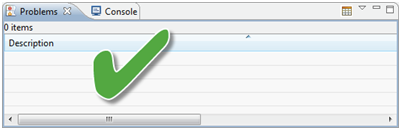
\includegraphics[width=0.5 \textwidth]{images/ProblemsView.png}}
    \vspace{-20pt}
    \caption{\label{fig:CodeWarrior-FereastraProblems} Când totul decurge bine...}
    \vspace{-10pt}
\end{wrapfigure}

Dacă totul a decurs cu bine, trebuie să nu avem erori în fereastra \textit{"Problems"}, așa cum evidențiază figura \ref{fig:CodeWarrior-FereastraProblems}. Această fereastră poate conține atât erori cât și warning-uri. Chiar dacă warning-urile nu împiedică procesul de building așa cum o fac erorile, este indicat să le luați în seamă pentru că ele pot evidenția alte probleme, ce apar la runtime (la rularea codului de pe placă).

\newpage

\section{Descărcarea codului pe placă}

\begin{wrapfigure}{r}{0.7\textwidth}
    \vspace{-25pt}
    \center{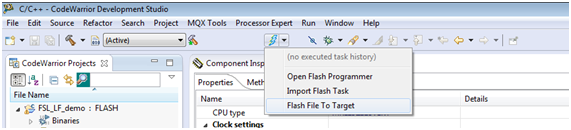
\includegraphics[width=0.7 \textwidth]{images/FlashProgrammer1.png}}
    \vspace{-20pt}
    \caption{\label{fig:CodeWarrior-FlashProgrammer1} Încărcarea codului pe placă}
    \vspace{-20pt}
\end{wrapfigure}

În urma compilării rezultă un executabil ce va trebui să fie flash-uit pe robot. Acest proces este realizat cu ajutorul unui instrument numit \textit{Flash Programmer}, iar figurile \ref{fig:CodeWarrior-FlashProgrammer1} și \ref{fig:CodeWarrior-FlashProgrammer2} vin să explice pașii ce trebuie urmăriți. Partea cea mai frumoasă o constituie faptul că aceste configurări vor fi făcute o singură dată. Ele sunt salvate local și pot fi refolosite de fiecare dată când este nevoie de ele.

\begin{wrapfigure}{r}{0.5\textwidth}
    \vspace{-70pt}
    \center{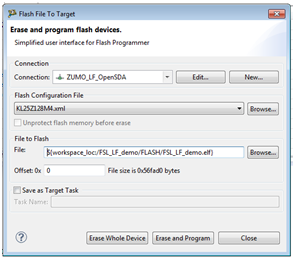
\includegraphics[width=0.5 \textwidth]{images/FlashProgrammer2.png}}
    \vspace{-20pt}
    \caption{\label{fig:CodeWarrior-FlashProgrammer2} Flash-uirea unui executabil}
    \vspace{-20pt}
\end{wrapfigure}

\section{Debugging}

Până să ajungeți la o versiune funcțională, pe care să o puteți prezenta la concurs sau în cercul vostru de prieteni, va fi ceva de munca. Lucrurile vor fi abordate pas cu pas, va trebui de multe ori să faceți un debugging avansat pentru a înțelege ce e greșit în algoritmul vostru de robotul nu face ceea ce doriți voi să facă. În cazul în care vreți să puteți executa programul în modul debug (pas-cu-pas), puteți folosi butonul exemplificat în figura \ref{fig:CodeWarrior-Debugging}. Nu uitați, pentru a folosi acest mod, robotul trebuie să rămână conectat la laptop printr-un cablu. Ca alternativa - recomandată, de altfel – puteți folosi interfața serială pentru a trimite date dinspre robot spre laptop.

\begin{wrapfigure}{l}{0.5\textwidth}
    \vspace{-20pt}
    \center{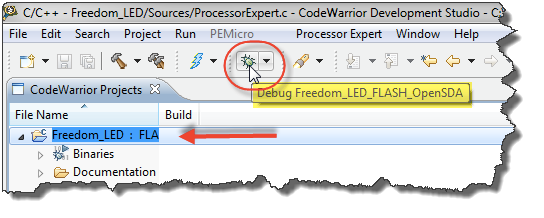
\includegraphics[width=0.5 \textwidth]{images/Debugging.png}}
    \vspace{-25pt}
    \caption{\label{fig:CodeWarrior-Debugging} Accesarea modului de debugging}
    \vspace{-20pt}
\end{wrapfigure}

Folosirea acestei interfețe seriale, vă va permite să faceți debugging folosind apeluri ale funcției \textit{printf}, cea mai primitivă metodă de a depana un program software. Din fericire, există și alte metode ceva mai avansate, cu rezultate mult mai bune, metode ce vor fi prezentate la ședințele tehnice.

\section{Processor Expert}

Processor Expert este un sistem de dezvoltare pus la dispozție de firma \textit{Freescale Semiconductor} ce poate regăsit deja instalat în \textit{odeWarrior for MCU}, prin intermediul căruia se pot crea și configura componente software ce generează cod sursă pentru microcontrollere produse de \textit{Freescale}. O astfel de componentă poate fi un driver, un algoritm sau o colecție de funcții software ce deservesc un obiectiv. O componentă poate fi, de exemplu, un driver ce permite accesul facil la pinii de intrare / ieșire puși la dispoziție de un microcontroller.

Folosirea Processor Expert înleșneste lucrul cu platforma hardware prin abstractizarea detaliilor de la nivelul low-level. Putem spune că avem de-a face cu o programare vizuală, în care este mai mult folosit mouse-ul decât tastatura. Noi, ca și programatori, vom avea mai multe de configurat setări și opțiuni pentru respectivul modul, pentru că mai apoi, codul să fie generat automat în funcție de inputul pe care l-am specificat. 

În cadrul acestui concurs, vom folosi Processor Expert. De ce? Răspunsul este foarte simplu. Cu ajutorul lui putem adăuga și configura componente, apoi genera cod sursă C pentru aceste componente. Codul generat va coexista cu codul C din proiectul nostru. Rezultatul acestei combinații de cod C scris manual și cel generat de \textit{Processor Expert} va fi compilat într-un singur executabil ce va fi folosit pentru construirea unui \textit{Line Follower}.

\subsection{Accesarea utilitarului}

\begin{wrapfigure}{r}{0.3\textwidth}
    \vspace{-60pt}
    \center{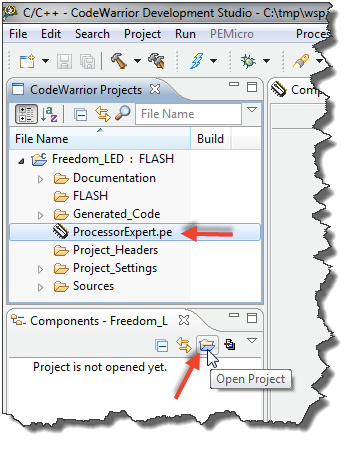
\includegraphics[width=0.3 \textwidth]{images/ProcessorExpert.png}}
    \vspace{-25pt}
    \caption{\label{fig:CodeWarrior-ProcessorExpert} Accesarea componentelor Processor Expert}
    \vspace{-50pt}
\end{wrapfigure}

După deschiderea proiectului în \textit{CodeWarrior for MCU}, în cazul în care fereastra \textit{Processor Expert} nu este vizibilă, va trebui să procedăm ca în figura \ref{fig:CodeWarrior-ProcessorExpert}.

\subsection{Adăugarea unei noi componente}

\begin{wrapfigure}{r}{0.3\textwidth}
    \vspace{-30pt}
    \center{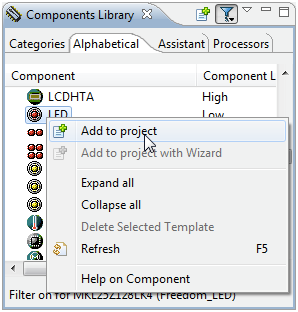
\includegraphics[width=0.3 \textwidth]{images/ProcessorExpertAdd.png}}
    \vspace{-20pt}
    \caption{\label{fig:CodeWarrior-ProcessorExpertAdd} Cum se adaugă o nouă componentă?}
    \vspace{-10pt}
\end{wrapfigure}

Înainte de a putea utiliza o componentă definită de acest utilitar, va trebui mai întâi, așa cum este și logic, să o adăugăm în cadrul proiectului nostru. Procesul de adăugare a unei componente este relativ simplu, fiind similar cu cel descris în figura \ref{fig:CodeWarrior-ProcessorExpertAdd}, din cadrul fereastrei de lucru \textit{Components Library}.

\subsection{Generarea de cod sursă}

După ce toate componentele necesare au fost adăugate și setate corect (sau după modificarea setaăilor unor componente) trebuie lansată o comandă prin care Processor Expert va fi înstiințat de faptul că trebuie să genereze codul sursă pentru componentele existente în proiect. Acest proces de înștiințare are loc doar prin apăsarea unui singur buton și anume - \textit{"Generate Processor Expert Code"}. După apăsarea butonului, utilitarul vă va rugă să aveți răbdare...

\textcolor{red}{Notă:} Codul generat de Processor Expert conține zone ca cele de mai jos, rezervate special pentru codul pe care voi îl veți scrie. Nu încercați ăa modificați sau să scrieți cod în afara acestor zone, deoarece o noua generare a codului Processor Expert vă va șterge tot ce ați adăugat. Iar asta nu este foarte plăcut, pentru că va trebui să o luați de la capăt cu acele modificări manuale.

\newpage

\begin{figure}[h!]
    \vspace{-10pt}
    \center{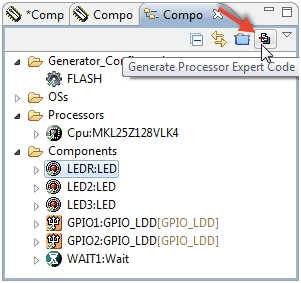
\includegraphics[width=0.3 \textwidth]{images/ProcessorExpertGenerate.png}}
    \vspace{-10pt}
    \caption{\label{fig:CodeWarrior-ProcessorExpertGenerate} Generarea de cod în Processor Expert}
    \vspace{-10pt}
\end{figure}

\lstinputlisting[caption=Inițializarea modulelor hardware, style=customc]{sources/generatingPExCode.lst}

% Configurarea componentelor Processor Expert
\chapter{Componente Processor Expert}

\label{sec:ProcessorExpert}

\section{Porturi de intrare și ieșire}

\begin{wrapfigure}{l}{0.5\textwidth}
    \vspace{-30pt}
    \center{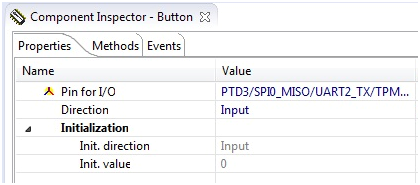
\includegraphics[width=0.5 \textwidth]{images/BitIO.png}}
    \vspace{-15pt}
    \caption{\label{fig:CodeWarrior-BitIO} Configurarea unui port de intrare / ieșire}
    \vspace{-10pt}
\end{wrapfigure}

Cu ajutorul componentei \textit{BitIO} din Processor Expert putem accesa porturi de intrare și iesire ale microcontroller-ului, folosind pinii configurabili ai acestuia. O astfel de componentă este caracterizată de un nume, de un pin al microcontrollerului pe care este mapată, o direcție (portul poate fi de intrare sau de ieșire) și valoarea inițiala, în cazul pinilor configurați pentru ieșire. Cu o astfel de componentă se poate controla foarte ușor un LED, spre exemplu.

\subsection{Porturi de ieșire}

\begin{wrapfigure}{r}{0.5\textwidth}
    \vspace{-60pt}
    \center{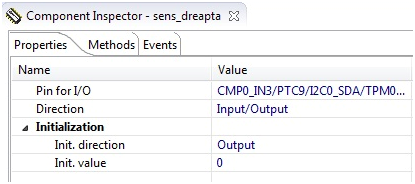
\includegraphics[width=0.5 \textwidth]{images/PExOutputIO.png}}
    \vspace{-20pt}
    \caption{\label{fig:CodeWarrior-PExOutputIO} Utilizarea unei componente}
    \vspace{-10pt}
\end{wrapfigure}

În figura \ref{fig:CodeWarrior-PExOutputIO} se poate regăsi un exemplu de utilizare al acestei componente. După cum vă puteți da seama, \textit{Init. direction} vine să specifice tipul portului, iar \textit{Init. value} valoarea inițială a acestuia.

Următoarele metode sunt puse la dispoziție pentru un programator în vederea controlării unui astfel de port:
\begin{description}
    \item[void SetVal(void), void ClrVal(void)] Acestea permit setarea portului de ieșire la valoarea \textit{"high"}, respectiv \textit{"low"}. 
    \item[void NegVal(void)] Metoda permite negarea unei valori setate ca output. Din 0 se poate se poate trece în 1 și invers. Cu ajutorul acestei metode se poate face un led, de exemplu, să blinkăie.
    \item[void PutVal(bool Val)] Metoda permite setarea valorii de ieșire pe un pin de ieșire.
    \item[void SetDir(bool Dir)] Setează direcția unui pin. Dacă parametrul are valoarea FALSE, pin-ul este marcat ca fiind pin de intrare (un buton, spre exemplu), iar dacă are valoarea TRUE, atunci el devine pin de ieșire.
\end{description}

De asemenea, mai jos avem și un exemplu simplu de utilizare al acestei componente:

\lstinputlisting[caption=Exemplu de utilizare a unui BitIO, style=customc]{sources/exampleBitIO.lst}

\subsection{Porturi de intrare}

Următoarele metode sunt puse la dispoziție pentru un programator în vederea controlării unui astfel de port:

\begin{description}
    \item[bool GetVal(void)] Întoarce valoarea pinului de intrare: FALSE pentru "0", respectiv TRUE pentru "1". În cazul unui buton, obținerea valorii "0" înseamnă că butonul este apăsat.
\end{description}

Citirea valorii unui port de intrare, se poate face într-o buclă infinită, așa cum arată exemplul următor:

\lstinputlisting[caption=Citirea stării unui buton în buclă, style=customc]{sources/exampleBitIORead.lst}

\newpage

\subsection{Componenta de așteptare (Wait)}

\begin{wrapfigure}{l}{0.5\textwidth}
    \vspace{-25pt}
    \center{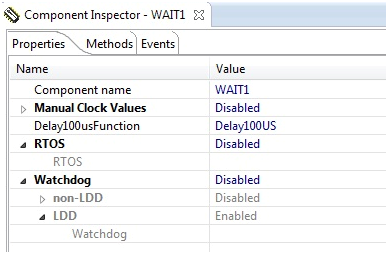
\includegraphics[width=0.5 \textwidth]{images/Wait.png}}
    \vspace{-20pt}
    \caption{\label{fig:CodeWarrior-Wait} Configurarea componentei Wait}
    \vspace{-10pt}
\end{wrapfigure}

Processor Expert pune la dispoziție o componentă ce implementează o rutină wait, prin intermediul căreia putem introduce o întârziere în cadrul execuției programului nostru. De exemplu, dacă vrem ca led-ul nostru să se aprindă și să se stingă la fiecare 5 secunde vom apela rutinele definite mai sus, secvențial, folosind ca și pas intermediar această componentă. În timp ce ne aflăm în această rutină de așteptare, doar întreruperile mai pot produce ieșirea din rutină. Ca și o mică paranteză, o întrerupere reprezintă un semnal sincron sau asincron de la un periferic ce semnalizează apariția unui
eveniment care trebuie tratat de către procesor. Tratarea întreruperii are ca efect suspendarea firului normal de execuție al unui program și lansarea în execuție a unei rutine de tratare a întreruperii (mai multe detalii puteți citi aici \cite{interupereBib}).

Mai jos sunt definite și explicate câteva dintre proprietățile acestei componente:

\begin{description}
    \item[Component Name] reprezintă numele sub care componenta se regăsește în codul sursă. Deoarece este foarte posibil ca, în cadrul aplicației noastre, să avem mai multe componente de același tip, numele va fi folosit ca diferențiator. În plus, ar mai trebui să știți că toate metodele unei componente sunt prefixate, în mod implicit, cu numele componentei de care aparțin.
    \item[Manual clock values] permite obținerea tactului de ceas fie de la CPU (opțiunea implicită, așa o vom folosi noi), fie de la o valoare specificată manual.
    \item[Delay100usFunction] menționează funcția ce furnizează o întârziere de 100 microsecunde. Se va folosi funcția specificată în imaginea de mai sus.
    \item[RTOS] este parametrul prin care componenta este informată dacă un sistem de operare este folosit în sistem (sistem de operare în timp real). În cazul nostru, ar reprezenta un overhead utilizarea unui sistem de operare, având în vedere că acesta ar fi util doar dacă avem o aplicație ce necesită support de multitasking.
\end{description}

Cum sistemul nostru nu folosește watchdogs, parametrul \textbf{WatchDog} trebuie configurat pe modul dezactivat. Un circuit watchdog este un circuit hardware concepute pentru a proteja un sistem electronic, în cazul în care ceva nu merge bine, iar sistemul nu poate recupera pe cont propriu (mai multe detalii despre un watchdog puteți găsi aici \cite{watchdogBib}).

Componenta poate fi folosită prin accesarea metodelor prezentate succint mai jos:

\begin{description}
    \item[void WaitCycles(word cycles)] parametrul specifică câți cicli de procesor se așteaptă;
    \item[void Waitms(word ms)] parametrul specifică câte milisecunde se va așteapta până la executarea următoarei instrucțiuni din programul nostru;
    \item[void Waitus(word us)] parametrul specifică câte microsecunde se așteaptă;
\end{description}

\textcolor{red}{Notă:} Există două clase de metode pentru componenta Wait. Unele permit specificarea numărului de secunde cât se așteaptă, celelalte operează cu cicli de ceas.

\subsection{Componenta Timer}

Folosind o componentă de tip \textit{Timer}, pusa la dispoziție de \textit{Processor Expert}, putem măsura ușor trecerea timpului. Timerul, după cum îi spune și numele, oferă facilitatea de a măsura intervale fixe de timp și de a genera întreruperi la expirarea intervalului măsurat. Un timer, odată inițializat va funcționa independent de unitatea centrală (core-ul microprocesorului). Acest lucru permite eliminarea buclelor de întârziere din programul principal.

Principiul de funcționare a unui \textit{Timer} poate fi descris în linii mari de cele trei unități:

\begin{enumerate}
    \item \textbf{Registrul numărător (Timer Counter)} - măsoară efectiv intervalele de timp și este incrementat automat cu o frecvență cunoscută.
    \item \textbf{Prescaler-ul} - are rolul de a diviza în funcție de necesitățile aplicației frecvența de ceas. În acest fel, registrul numărător poate fi incrementat mai repede sau mai încet.
    \item La fiecare incrementare a TCNT are loc o comparație între acest registru și o valoare stocată într-un alt registru - numit registru comparator. Valoarea din registrul comparator poate fi încărcată de către programator prin scrierea lui. Dacă are loc egalitatea se generează o întrerupere, în caz contrar incrementarea continuă.
\end{enumerate}

\begin{wrapfigure}{r}{0.5\textwidth}
    \vspace{-30pt}
    \center{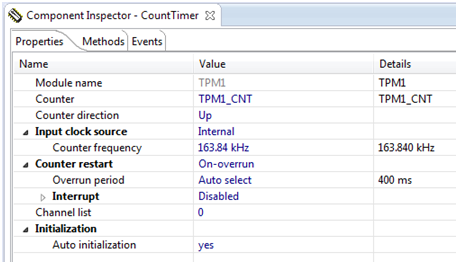
\includegraphics[width=0.5 \textwidth]{images/Timer.png}}
    \vspace{-20pt}
    \caption{\label{fig:CodeWarrior-Timer} Configurarea unui timer}
    \vspace{-10pt}
\end{wrapfigure}

Timerele sunt prevăzute cu mai multe canale astfel încât se pot desfășura diferite număratori în paralel. Vă invităm să vă documentați asupra numărului de timere și de canale pe care placa de dezvoltare FRDM-KL25Z le pune la dispoziție, pentru că aceasta este placa pe care veți dezvolta aplicația. De asemenea, timerele pot funcționa și în moduri PWM, astfel încât să genereze pe un pin de ieșire un semnal. Mai multe detalii veți afla în paragrafele următoare.

Proprietăți ale componentei:

\begin{description}
    \item[Component Name] reprezintă numele sub care componenta se regăsește în codul sursă.
    \item[Counter Direction] permite specificarea direcției în care se numără: registrul numărător se incrementează sau se va decrementa?
    \item[Counter Frequency] definește granularitatea cu care se numără. Numărătorul incrementeaza valoarea counter-ului în funcție de această frecvență. De exemplu, dacă setăm frecvența la 1 kHz, într-o secundă, numărătorul ajunge la valoarea 1000. 
\end{description}

Metode de interfațare:

\begin{description}
    \item[$LLD\_Error$ ResetCounter(LDD\_TDeviceData *DeviceDataPtr)] inițializează la 0 (resetează) counter-ul. În cazul proiectului nostru, parametrul \textit{DeviceDataPtr} poate fi setat la \textit{NULL}. Funcția întoarce ERR\_OK dacă totul a decurs bine și ERR\_SPEED în caz de eroare. 
    \item[TValueType GetCounterValue(LDD\_TDeviceData *DeviceDataPtr)] această funcție returnează valoarea registrului contor (numărul de pulsuri de ceas înregistrate de la ultima operație de \textit{Reset}). În cazul proiectului nostru, parametrul \textit{DeviceDataPtr} poate fi setat pe NULL.
\end{description}

Iată și un exemplu simplu de utilizare:

\lstinputlisting[caption=Utilizarea unui Timer, style=customc]{sources/exampleTimer.lst}

\subsection{Componenta PWM (Pulse Width Modulation)}

\textit{PWM (Pulse Width Modulation)} este o tehnică folosită pentru a varia în mod controlat tensiunea dată unui dispozitiv electronic. Această metodă schimbă foarte rapid tensiunea oferită dispozitivului respectiv din \textit{ON} în \textit{OFF} și invers. Perioada de timp corespunzătoare valorii ON dintr-un ciclu ON-OFF se numește factor de umplere (în engleză - \textit{duty cycle}) și reprezintă, in medie, ce tensiune va primi dispozitivul electronic. Astfel, se pot controla circuitele analogice din domeniul digital. Practic, asta înseamnă că un LED acționat astfel se va putea aprinde / stinge gradual, iar în cazul unui motor acesta se va roti mai repede sau mai încet.

Factorul de umplere se exprimă în procente și reprezintă cât la sută din perioada unui semnal acesta va fi pe nivelul ON. Modularea folosește variația factorului de umplere a unei forme de undă dreptunghiulară pentru a genera la ieșire o tensiune analogică. Așadar, putem control o variabilă prin intermediul alteia. De exemplu, putem controla amplitudinea unei sinusoide (numită purtătoare) cu un alt semnal (rezultând modulatie în amplitudine - AM). A nu se confunda cu combinarea (mixarea) a două semnale, unde semnalele sunt pur și simplu adunate.

\begin{figure}
    \centering
    \subfloat[]{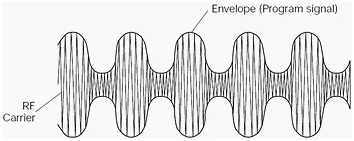
\includegraphics[width=3.1in]{images/Modulation1.png}} 
    \subfloat[]{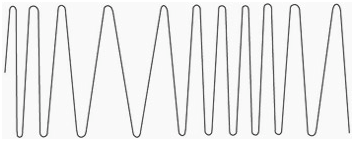
\includegraphics[width=3.1in]{images/Modulation2.png}}
    \caption{Modulație în amplitudine (a) și în frecvență (b)} 
    \label{fig:CodeWarrior-Modulation} 
\end{figure} 

\subsubsection{Modificarea turației unui motor}

\begin{wrapfigure}{r}{0.3\textwidth}
    \vspace{-20pt}
    \center{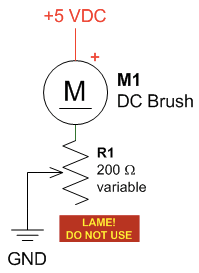
\includegraphics[width=0.3 \textwidth]{images/ResistenceMethod.png}}
    \vspace{-15pt}
    \caption{\label{fig:CodeWarrior-ResistenceMethod} Controlarea unui motor folosind o rezistență}
    \vspace{-10pt}
\end{wrapfigure}

Să presupunem că avem un motor ce funcționează la o anumită tensiune, în curent continuu. Aplicându-i acea tensiune, motorul va funcționa la o anumită turație. Ce facem dacă vrem să-i modificăm turația? O variantă este să folosim roți dințate, dar dacă am vrea să-l controlam prin metode electrice? Cea mai simpla (și ineficientă) formă de a controla turația unui motor în curent continuu este folosirea unei rezistențe. Este ineficientă deoarece multă energie este pierdută, transformându-se în căldură.

Dacă înlocuim rezistența cu un tranzistor, putem controla turația (viteza) motorului aplicând în baza tranzistorului un semnal - cât timp semnalul este "high", tranzistorul închide circuitul motorului către masă. Când semnalul din baza tranzistorului este pe "low", prin motor nu trece curent. Pierderi de putere apar acum (față de exemplul anterior, în care foloseam o rezistență) doar la trecerea între semnalul "high" și cel "coborât" - iar timpul petrecut în aceste faze tranzitorii este foarte scurt.

\begin{wrapfigure}{r}{0.3\textwidth}
    \vspace{-60pt}
    \center{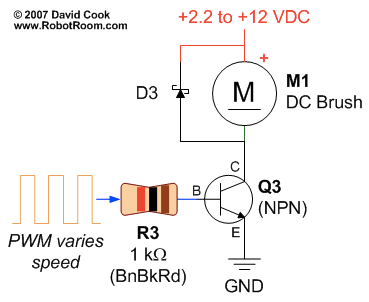
\includegraphics[width=0.3 \textwidth]{images/TransistorMethod.png}}
     \vspace{-15pt}
    \caption{\label{fig:CodeWarrior-TransistorMethod} Controlarea unui motor folosind un tranzistor}
    \vspace{-10pt}
\end{wrapfigure}

Motorul are o anumită inerție, astfel încât nu pornește sau se oprește brusc. De aceea, controlarea tranzistorului printr-un semnal drepunghiular cu o frecvență suficient de mare (semnificativ mai mare decât timpul de răspuns al motorului) nu produce "smucituri" în funcționarea motorului. În același mod putem controla intensitatea luminii generate de un led. Ca și o curiozitate, dacă folosim în baza tranzistorului o frecvență în spectrul auzului uman, vom sfârși prin a auzi un bazâit. De aceea, dacă este posibil, e bine ca frecvența folosită să fie peste 20 kHz. Și nu uitați de câini, care aud la frecvențe și mai mari de 20 kHz!

\subsubsection{Generarea unui semnal PWM în mediu digital}

Majoritatea microcontrollerelor pot genera semnale PWM (pe un pin de ieșire) folosind un numărător ce este incrementat automat cu o anumita cadență până ajunge la o anumită valoare - când este resetat și procesul se reia. Într-o astfel de perioadă, semnalul pe pinul de ieșire este "low" (sau "high") până când numărătorul ajunge la o valoare și apoi este comutat în cealaltă stare. În acest fel creăm un semnal dreptunghiular, cu care vom controla motorul.

\begin{wrapfigure}{r}{0.5\textwidth}
    \vspace{-20pt}
    \center{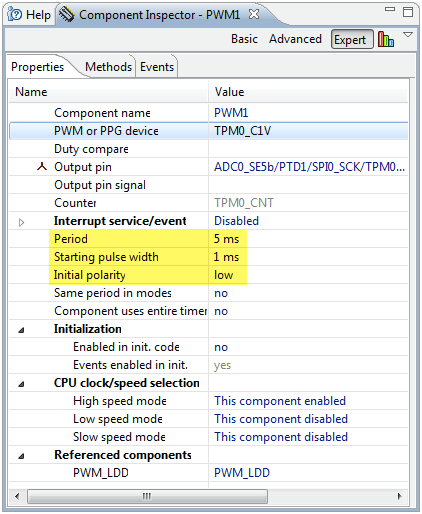
\includegraphics[width=0.5 \textwidth]{images/PExPWM.png}}
    \vspace{-15pt}
    \caption{\label{fig:CodeWarrior-PExPWM} Configurarea unei componente de tip PWM}
    \vspace{-30pt}
\end{wrapfigure}

\subsubsection{Processor Expert și generarea de semnal PWM}

Proprietăți ale componentei:

\begin{description}
    \item[Component Name] element de identificare al componentei;
    \item[Output Pin] este pinul fizic pe care este mapată componentă;
    \item[Period] în mod evident, reprezintă perioada semnalului PWM;
    \item[Starting Pulse Width] este timpul setat pentru prima parte din duty cycle; 
    \item[Initial Polarity] definește dacă prima parte a duty cycle-ului este ON sau OFF;
    \item[Initialization] specifică dacă la inițializare / resetare componenta este sau nu activată. Dacă nu este activată, ieșirea pe pin este setată la valoarea definită prin \textit{"Initial Polarity"}. În acest caz, pentru a o activa programatic, trebuie folosită metoda \textit{Enable}; 
\end{description}

\textcolor{red}{Notă:} Pentru modificarea programatică a duty cycle-ului, Processor Expert pune la dispoziție mai multe metode, noi folosind \textbf{void SetRatio16(word ratio)}.

Metode de interfațare:

\begin{description}
    \item[byte Enable / Disable (void)] metodele pornesc / opresc componenta (generarea de semnal). Valoarea întoarsă poate fi ERR\_OK sau ERR\_SPEED.
    \item[byte SetRatio16(word ratio)] aceasta metodă setează un nou duty cycle pentru componentă. Ratio este o valoare unsigned, cuprinsă între 0x0 și 0xffff (65535), proporțională cu procentul 0 - 100\%. Valoarea întoarsă poate fi ERR\_OK sau ERR\_SPEED.
    \item[byte SetValue(void), byte ClrValue(void)] permit setarea directă a pinului de ieșire atunci când componenta este oprită (folosind metoda \textit{Disable}, în prealabil). Valoarea întoarsă poate fi ERR\_OK, ERR\_SPEED sau ERR\_ENABLE.
\end{description}

O dată instanțiată o componentă de acest tip, funcțiile oferite pot fi folosite așa cum sunt utilizate mai jos:

\lstinputlisting[caption=Utilizarea funcțiilor puse la dispozție de componenta PWM, style=customc]{sources/examplePWM.lst}

\subsubsection{Controlul sensului de rotație al motorului}

Cu ajutorul unui semnal PWM putem modula viteza de rotație a unui motor. Este important, de asemenea, să controlăm și sensul în care motorul se rotește. Acest lucru îl vom realiza prin intermediul unui pin de ieșire al microprocesorului conectat la fiecare punte H ce comanda un motor. În funcție de valoarea acestui pin (0 sau 1) stabilim direcția în care se învârte motorul.

\subsubsection{Logică inversată}

Placa de dezvoltare FRDM-KL25Z și motoarele folosite în cadrul acestui proiect funcționează după o logică inversată. Îți aduci aminte ce înseamna "duty cycle"? Dacă nu, îți mai aducem noi aminte încă o dată, însemna că viteza motorului era mai mare cu cât semnalul nostru stătea mai mult timp în "high" (1 logic) într-o perioada. Ehh, gândeste-te acum exact invers – în loc să conteze cât stă în "high", contează cât stă în "low" (0 logic).



% Cateva informatii despre componentele hardware utilizate
\chapter{Interacțiunea cu mediul extern}

\section{Interfața serială}

Este foarte probabil ca mulți dintre voi să fi depanat până acum un program software doar prin folosirea metodei clasice și probabil cea mai simplă și intuitivă - folosirea \textit{printf-urilor} (limbajul C) sau a \textit{cout-urilor} dacă sunteți familarizați cu C++. Dacă în cadrul unei aplicați software clasice, ieșirea programului este redată pe un monitor, în cadrul unei aplicații embedded nu avem un astfel de dispozitiv. Cel mult vom avea un LCD. În acest caz, ne propunem să trimitem aceste date către un calculator persoanal prin care le-am putea accesa cu ușurință. Soluția este folosirea unei interfețe seriale. Configurația oferită de către proiectul inițial (folosind \textit{Processor Expert}) are deja configurat[ interfața serială de pe microcontroller.

Aceasta poate fi folosita din programul dezvoltat pe microcontroller prin apelul următoarelor funcții:

\begin{description}
    \item[void Term1\_SendChar(char\_t Val)] Realizează transmiterea unui singur caracter.
    \item[void Term1\_SendStr(void *str)] Util pentru transmiterea unui șir de caractere (a unui string).
    \item[void Term1\_SendNum(int32\_t number)] Util pentru transmiterea unui număr întreg (reprezentat pe 32 de biți).
\end{description}

\begin{figure}[h!]
  \vspace{-10pt}
  \center{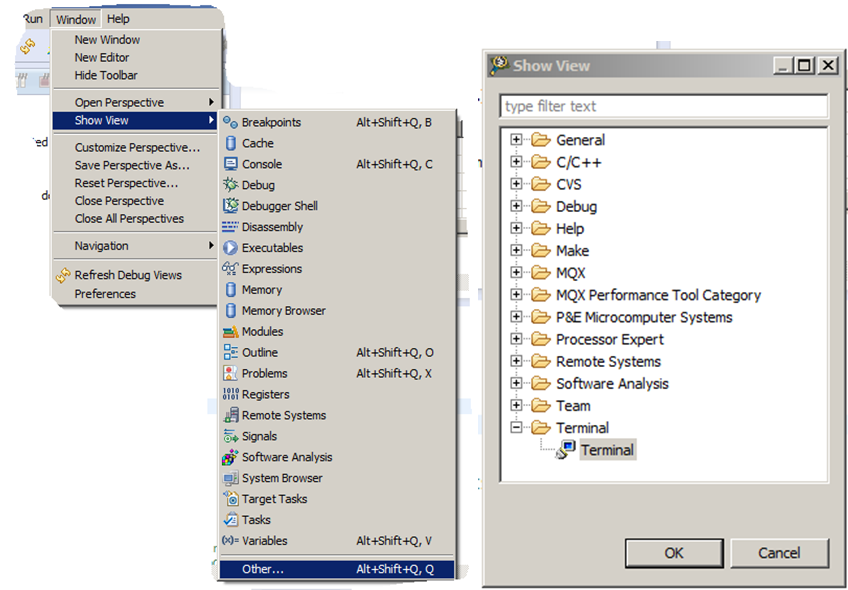
\includegraphics[width=0.8 \textwidth]{images/EclipseTerminal.png}}
  \vspace{-5pt}
  \caption{\label{fig:CodeWarrior-EclipseTerminal} Accesarea terminalului pus la dispoziție de Eclipse}
  \vspace{-10pt}
\end{figure}

În mediul de dezvoltare (Eclipse) se poate folosi un terminal pentru a recepționa datele transmise de către microcontroller prin interfața serială. Acest terminal va trebui accesat ca în figura.

Terminalul va apărea în partea de jos a ecranului în taburile de console. Pentru o comunicare corectă (pentru că terminalul să înțeleagă corect datele trimise), terminalul trebuie configurat după cum urmează:

Portul selectat trebuie să fie portul pe care s-a atașat \textit{OpenSDA} (în Windows, poate fi verificat în \textit{"Device Manager"}, mai exact în \textit{"Ports (COM \& LPT)"}). După configurare, terminalul va trebui conectat la portul cu care comunică. Aceasta se face prin simpla apăsare a butonului de conectare (primul din lista de butoane de tip iconițe ale ferestrei "Terminal" ce apare în partea de jos a Eclipse-ului).

\section{Senzori cu infraroșu}

Pentru a putea detecta diferența dintre linia neagră și fundalul alb al traseului, robotul \textit{Zumo} folosește o matrice de senzori cu infraroșu. Acești senzori pot măsura cantitatea de lumina reflectată de diferite suprafațe, în funcție de proprietățile acesteia. Cum funcționează? Foarte simplu. O diodă emite radiații în spectrul infraroșu spre suprafața din dreptul senzorului și o parte mai mică sau mai mare din această lumina va fi absorbită de suprafață. Ce ne interesează pe noi este cantitea de lumina reflectată ce va fi masurată cu ajutorul unui fototranzistor și al unui condensator.

\begin{wrapfigure}{l}{0.5\textwidth}
    \vspace{-20pt}
    \center{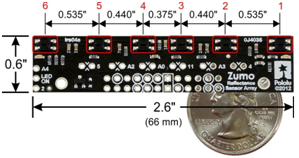
\includegraphics[width=0.5 \textwidth]{images/InfraredSensors.png}}
    \vspace{-15pt}
    \caption{\label{fig:CodeWarrior-InfraredSensors} Bareta de senzori}
    \vspace{-20pt}
\end{wrapfigure}

După cum îi spune și numele, matricea de senzori este alcătuită din mai multe elemente. Acest lucru este necesar deoarece fiecare senzor poate măsura doar cantitatea de lumina care este reflectată din jurul său (pe o arie redusă ca și suprafață). Bareta care este pusă la dispoziție pentru robotul Zumo are 6 astfel de elemente pentru detecția liniei negre. Aceasta este amplasată sub lama robotului, asigurându-se o protecție atât mecanică cât și o reducere a cantității de lumina ambientală care poate duce la perturbarea măsurătorilor.

Ieșirea senzorilor este dată de durata ($T$) a unui impuls electric. Cu cât impulsul este mai de durată, cu atât cantitatea de lumina reflectată este mai mică.

Următoarele componente \textit{Processor Expert} vor fi folosite în interfațarea cu acești senzori:

\begin{itemize}
    \item intrările / ieșirile digitale (componente de tip \textit{BitIO}): A1, A3, D11, A0, A2, D5, IR\_LED;
    \item un timer (componentă de tip \textit{TimerUnit\_LDD}) CountTimer;
    \item componentă necesară adăugării unui întârzieri - \textit{WAIT1};
\end{itemize}

Pașii necesari pentru obținerea unei iterații de date despre mediu, de la senzori, ar fi următorii:

\begin{enumerate}
    \item Activăm diodele infraroșii - IR\_LED.
    \item Configurăm pinii digitali (A1, A3, D11, A0, A2, D5) ca ieșiri și le setăm pe valoarea 1.
    \item Așteptăm o perioadă de timp astfel încât condensatorul să se încarce - 50 µs este suficient.
    \item Configurăm pinii de la pasul 2 ca intrări digitale, de această dată.
    \item Resetăm timer-ul \textit{CountTimer}. După inițializare acestă funcționează în continuu astfel avem nevoie de o resetare a timpului măsurat până atunci – nu se știe starea în care va fi găsit. Timer-ul măsoară perioade de timp în multipli de 6.10 µs (163.84kHz).
    \item Măsurăm timpul necesar ca tensiunea de pe condensator să comute intrările în valoarea 0. După o perioadă de câteva µs, senzorii pot fi considerați ca au toți valoarea 0. Acest mecanism ne permite să reducem perioada de așteptare între citiri, după un anumit prag (perioadă) nu se mai obține informatii utile de la senzori.
    \item Dezactivăm diodele infraroșii.
\end{enumerate}

% Sectiunea de referinte va fi mereu pe o alta pagina
\newpage

% Dezvoltarea unei aplicatii in CodeWarrior for MCU
% Redenumim anumite comenzi
\renewcommand*{\refname}{Referințe bibliografice}

% Referinte...
\begin{thebibliography}{00}
\bibitem{} http://en.wikipedia.org
\bibitem{} http://en.wikibooks.org/wiki/Embedded\_Systems/Super\_Loop\_Architecture
\bibitem{} http://mcuoneclipse.com/2012/09/07/tutorial-enlighting-the-freedom-kl25z-board
\bibitem{} http://electrical-engineering-portal.com/what-is-modulation
\bibitem{} http://mcuoneclipse.com/2013/03/16/pwm-for-processor-expert-explained
\bibitem{interupereBib} http://andrei.clubcisco.ro/cursuri/3pm/lab2.pdf
\bibitem{watchdogBib} http://en.wikipedia.org/wiki/Watchdog\_timer
\bibitem{} http://www.freescale.com/webapp/sps/site/prod\_summary.jsp?code=FRDM-KL25Z\&fpsp=1\&tab=Documentation\_Tab
\end{thebibliography}

% Se adauga si pagina de bibliografie la cuprins
\addcontentsline{toc}{chapter}{Bibliografie}

% Sfarsitul documentului
\end{document}